\section{Introduction}

\frame[<+->]{
	\frametitle{Probability review}
	
	\begin{itemize}
	\item The \cblue{sample space} is the set of all possible outcomes of the experiment denoted by $\Omega$. \\
	For example, two successive coin tosses the sample space of \{hh, tt, ht, th\}, where $h$ heads and $t$ tails.

	\item A \cblue{event space} is a set whose elements $A  \in  F$ (called events) are subsets of $\Omega$ (i.e., $A \subseteq \Omega$ is a collection of possible outcomes of an experiment)
	\item  Probability measure $A$ function $P : F \to \Re$, we associate a number $P(A)$ that measures the
probability or degree of belief that the event will occur.
    \item satisfies the following properties:
    \begin{itemize}
    \item $P(A) \geq 0$
    \item$ A_1$, $A_2$, . . . are disjoint events (i.e. $A_i \cap A_j = \emptyset$ whenever $i \neq j$), then \\
    $P(\bigcup_i A_i) = \sum_i P(A_i)$
    \item $P(\Omega) = 1$
    \end{itemize}
     
	\end{itemize}

}

\frame[<+->]{
	\frametitle{}
	\begin{block}{Example}
	Consider the event of tossing a six-sided die. The sample space is $\Omega = \{1, 2, 3, 4, 5, 6\}$. We can define the simplest event space $F = \{\emptyset, \Omega\}$. Another event space is the set of all subsets of $\Omega$. \\
	For the first event space, the probability measure is given by $P(\emptyset) = 0$, $P(\Omega) = 1$. \\
	For the second event space, one valid probability measure is to assign the probability of each set in the event space to be $\frac{i}{6}$ where $i$ is the number of elements of that set; for example, $P(\{1, 2, 3, 4\}) = \frac{4}{6}$ and $P(\{1, 2, 3\}) = \frac{3}{6}$
	\end{block}
	



}


\section{PGM}
\frame[<+->]{
	\frametitle{Conditional probability}
	\begin{itemize}
	\item Let $B$ be an event with non-zero probability. \\
	The conditional probability of any event $A$ given $B$ is defined as:
	\begin{equation}
		\begin{aligned}
		P(A \mid B) = \frac {P(A, B)}{P(B)}
		\end{aligned}
	\end{equation}

	\item $P(A \mid B)$ is the probability measure of the event $A$ after observing the occurrence of event $B$.
	\end{itemize}
	


}

\frame[<+->]{
	\frametitle{Chain rule}
	\begin{itemize}
	\item Let  $S_1, \cdots, S_k$  be events, $P(S_i) >0$. Then the chain rule:
		\begin{equation}
		\begin{aligned}
 		 	& P(S_1, S_2 ,\cdots , S_k) \\
 		 	 =& P(S_1) P(S_2 | S_1) P(S_3 | S_2 , S_1 ) \cdot  P(S_k | S_1 , S_2 , \cdot S_{k-1})
		\end{aligned} 
	\end{equation}
	\item  With $k=2$ events, this is the definition of conditional probability:
	\begin{equation}
	\begin{aligned}
	P(S_1 , S_2) = P(S_1) P(S_2 | S_1)
	\end{aligned}
	\end{equation}

	\item In general, the chain rule is derived by applying the definition of conditional probability multiple times, for example:
	\begin{equation}
	\begin{aligned}
  & P(S_1 , S_2 , S_3,S_4) \\
=& P(S_1, S_2 , S_3) P(S_4 \mid S_1 , S_2 , S_3) \\
=& P(S_1 , S_2) P(S_3  \mid S_1, S_2) P(S_4  \mid S_1, S_2 , S_3) \\
=& P(S_1) P(S_2 \mid S_1) P(S_3 \mid S_1 , S_2) P(S_4 \mid S_1 , S_2 , S_3)
\end{aligned}
	\end{equation}

	\end{itemize}
	


}


\frame[<+->]{
	\frametitle{Independence  }
	\begin{itemize}
	\item Two events are called independent if and only if \\
	$P(A , B) = P(A)P(B)$, or $P(A \mid B) = P(A)$
	\item Thus, independence is equivalent to saying that observing $B$ does not have any effect on the probability of $A$
	\end{itemize}


}


\frame[<+->]{
	\frametitle{Random variables}
	\begin{itemize}
	\item We flip 10 coins, and we want to know the number of coins that come up heads.\\
	 The sample space $\Omega$ are 10-length sequences of heads and tails. For example, we might have $\omega_0 = \langle H, H, T, H, T, H, H, T, T, T \rangle \in \Omega$.
	 \item we care about real-valued functions of outcomes, the number of heads that appear among our 10 tosses. \\ These functions are known as \cblue{random variables}.

\item A random variable $X$ is a function $X : \Omega \to \Re$. 
\item We will denote random variables using upper case letters $X$ 
\item We will denote the value that a random variable may take on using lower case letters $x$. \\
Thus, $X = x$ means that we are assigning the value $x \in \Re$ to the random variable $X$
	\end{itemize}


}


\frame[<+->]{
	\frametitle{Cumulative distribution functions}
	\begin{itemize}
	\item To specify the probability measures used with random variables, it is convenient to specify alternative functions (\cblue{CDFs}, \cblue{PDFs}, and \cblue{PMFs}).
	\item A cumulative distribution function (CDF) is a function $F_X : \Re \to [0, 1]$ which specifies a probability measure as,\\
	\begin{equation}
	\begin{aligned}
	F_X(x) = P(X \leq x)
	\end{aligned}
	\end{equation}
	\item Properties:
	\begin{equation}
	\begin{aligned}
	& 0 \leq  F_X(x) \leq  1 \\
  & \lim_{x \to -\infty} F_X(x) = 0 \\
  & \lim_{x \to +\infty} F_X(x) = 1 \\
  & x \leq y \leftarrow  F_X(x) \leq F_X(y)
	\end{aligned}
	\end{equation}
	
	\end{itemize}


}

\frame[<+->]{
	\frametitle{Probability mass functions}
	\begin{itemize}
	\item When a random variable $X$ takes on a \cblue{finite} set of possible values  is a discrete random variable
	\item  A way to represent the probability measure associated with a random variable is to directly specify the probability of each value that the random variable can assume a probability mass function \cblue{PMF} is a function
	\item  $p_X : \Omega \to \Re$ such that $p_X(x) = P(X = x)$

\item Properties:
\begin{equation}
\begin{aligned}
0 \leq p_X(x) & \leq 1 \\
 \sum_{x \in X} p_X(x) & = 1 \\
\sum_{x \in A} p_X(x) & = P(X \in A)
\end{aligned}
\end{equation}

	\end{itemize}


}


\frame[<+->]{
	\frametitle{Probability density functions}
	\begin{itemize}
	\item For some continuous random variables, the cumulative distribution function $F_X(x)$  is differentiable everywhere. \\
	In these cases, we define the Probability Density Function or \cblue{PDF} as the derivative of the CDF
	\begin{equation}
	\begin{aligned}
	f_X(x) = \frac{dF_X(x)}{dx}
	\end{aligned}
	\end{equation}

	\item Properties:
	\begin{equation}
	\begin{aligned}
	f_X(x) & \geq 0 \\
  	\int^{\infty}_{-\infty} f_X(x) & = 1 \\
  	\int_{x \in A} f_X(x) dx & = P(X \in A)
	\end{aligned}
	\end{equation}

	\end{itemize}


}

\frame[<+->]{
	\frametitle{Expectation}
	\begin{itemize}
	\item $X$ is a discrete random variable with \cblue{PMF} $p_X(x)$ and $g : \Re \to \Re$ is an arbitrary function.
	\item  In this case, $g(X)$ can be considered a random variable, and we define the \cblue{expectation}> of $g(X)$  as
	\begin{equation}
	\begin{aligned}
	\E[g(X)] = \sum_{x \in X} g(x)p_X(x)
	\end{aligned}
	\end{equation}
	\item If $X$ is a continuous random variable with PDF $f_X(x)$, then the expected value of $g(X)$ is defined as:
	\begin{equation}
	\begin{aligned}
	\E[g(X)] = \int^{\infty}_{-\infty} g(x)f_X(x)dx
	\end{aligned}
	\end{equation}

	

	\end{itemize}


}

\frame[<+->]{
	\frametitle{Expectation}
	\begin{itemize}
	\item Intuitively, the expectation of $g(X)$ can be thought of as a \cblue{weighted average} of the values that $g(x)$ can taken on for different values of $x$, where the weights are given by $p_X(x)$
	\item Properties:
	
	\begin{equation}
	\begin{aligned}
	& \E[a] = a \text{for any constant}  a \in \Re \\
   	& \E[af(X)] = a\E[f(X)] \text{for any constant} a \in \Re \\
  	& \text{Linearity of Expectation} \E[f(X) + g(X)] = \E[f(X)] + \E[g(X)] 
	\end{aligned}
	\end{equation}

	\end{itemize}


}

\frame[<+->]{
	\frametitle{Discrete random variables}
	\begin{itemize}
	\item $X \sim \text{Bernoulli}(p)$ (where $0 \leq p \leq 1$): \\
	 one if a coin with heads probability $p$ comes up heads, zero otherwise
	\begin{equation}
	\begin{aligned}
	p(x)=\begin{cases}
    		p, & \text{if }x = 1. \\
    		1-p, & \text{if }x = 0.
	\end{cases} 
	\end{aligned}
	\end{equation}
	\item $X \sim \text{Binomial}(n, p)$ (where $0 \leq  p \leq  1$):\\
	 the number of heads in $n$  independent flips of a coin with heads probability $p$
	\begin{equation}
	\begin{aligned}
	 p= \binom{n}{x} \cdot p^x (1-p)^{n-x}
	 \end{aligned}
	\end{equation}
			 
	\end{itemize}


}


\frame[<+->]{
	\frametitle{Discrete random variables}
	\begin{itemize}
	
	\item $X \sim \text{Geometric}(p)$ (where $p > 0$):\\
	 the number of flips of a coin with heads probability $p$ until the first heads.
	 \begin{equation}
	 \begin{aligned}
	 p(x) = p(1 - p)^{x-1}
	 \end{aligned}
	 \end{equation}
	\item $X \sim \text{Poisson}(\lambda)$  (where $\lambda > 0$):\\
	 a probability distribution over the non-negative integers used for modelling the frequency of rare events.	
	\begin{equation}
	 \begin{aligned}
	 p(x) = e^{-\lambda} \frac{\lambda^x}{x!}
	  \end{aligned}
	\end{equation}		 
	\end{itemize}


}


\frame[<+->]{
	\frametitle{Continuous random variables}
	\begin{itemize}
	
	\item $X \sim \text{Uniform}(a, b)$ (where $a < b$): \\
	equal probability density to every value between $a$ and $b$ on the real line
	\begin{equation}
	\begin{aligned}
	f(x)=\begin{cases}
    \frac{1}{b-a}, & \text{if }a \leq b \\
    0, & \text{otherwise}
	\end{cases}
	\end{aligned}
	\end{equation}
	\item $X \sim \text{Exponential}(\lambda)$ (where $\lambda > 0$): \\
	decaying probability density over the non-negative real
	\begin{equation}
	\begin{aligned}
	f(x)=\begin{cases}
    \lambda e^{-\lambda x}, & \text{if }x \geq 0 \\
    0, & \text{otherwise}
	\end{cases}
	\end{aligned}
	\end{equation}
	\item $X \sim \text{Normal}(\mu, \sigma^2)$: also known as the Gaussian distribution
	\begin{equation}
	\begin{aligned}
	f(x) = \frac{1}{\sqrt{2\pi}\sigma}e^{-\frac{(x-\mu)^2}{2\sigma^2}}
	\end{aligned}
	\end{equation}
		 
	\end{itemize}


}

\frame[<+->]{
	\frametitle{Random variable example}
	\begin{itemize}
	\item We cannot talk about the exact value of the random variable but we can reason about it's possible values
	\item We quantify the degree of belief we have in each outcome
	\item \cblue{Uniform distribution}: every outcome is equally likely\\
	 if $n$ is the size of the set of possible outcomes the probability that $x$ takes on any value (e.g. a) is $\frac{1}{n}$
	 	\begin{equation}
	\begin{aligned}
	p(x) = \frac{1}{n} \text{for all} x \in [a,b]
	\end{aligned}
	\end{equation}
	\begin{figure}
	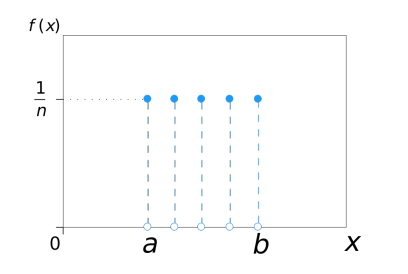
\includegraphics[scale=0.5]{uniform}
	\end{figure}
	
	\end{itemize}
	
	
}

\frame[<+->]{
	\frametitle{Random variable example}
	\begin{itemize}
	\item A random variable is a function it maps from a sample space $\Omega$ to $\Re$ \\
			$x : \Omega \rightarrow \Re$
	\item Example: which pet do kids love the most? \\
			Sample space: $\Omega =$ \{bird, cat, dog\}
			
				\begin{equation}
	\begin{aligned}
	 x(\omega)=\begin{cases}
   	1 &\omega = {bird}  \\
    2 &\omega = {cat}  \\
    3 &\omega = {dog}  \\
	\end{cases}
	\end{aligned}
	\end{equation}
	\item  if say $x$ we mean the set of outcomes	 \\
	${\omega : x() = x}$ which is called an event
	\item we call $\mathcal{X}$ the support of $X$
	\begin{figure}
	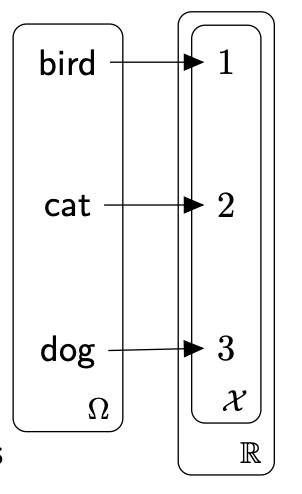
\includegraphics[scale=0.3]{support}
	\end{figure}
	
	\end{itemize}
	
	
}


\frame[<+->]{
	\frametitle{Random variable example}
	\begin{itemize}
	\item A Categorical variable can model $1$ of $k$ categories \\
		$x \sim \text{Cat}(\theta_1, . . . , \theta_k )$
	\item $x = {1, . . . , k}$
	\item the categorical parameter is a probability vector
	
	\begin{equation}
	\begin{aligned}
	0 \leq  \theta_x  & \leq  1 \text{for} x \in [1, k] \\
	\sum_{x=1}^{k} \theta_x & = 1
	\end{aligned}
	\end{equation}
	
	\begin{figure}
	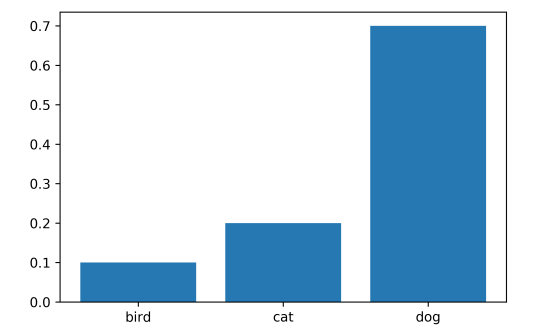
\includegraphics[scale=0.5]{cat}
	\end{figure}
	
	\end{itemize}
	
	
}



I 

\frame[<+->]{
	\frametitle{Sum rule and product rule}
	\begin{itemize}
	\item  $p(x, y)$ is the joint distribution of two random variables $x, y$.\\
	 With the corresponding marginal distributions $p(x)$ and $p(y)$
	 \item $p(y | x)$ is the conditional distribution of $y$ given $x$.
	 \item We denote the sum rule as (also known as the marginalization property):
		\begin{equation}
	\begin{aligned}
	 p(x)=\begin{cases}
    \sum_{y \in Y} p(x,y), & \text{if} y \text{is discrete} \\
    \int_{Y} p(x,y)dy, & \text{if} y \text{is continuous}
	\end{cases}
	\end{aligned}
	\end{equation}
	\item We sum out (or integrate out) the set of states $y$ of the random variable $Y$.
	\end{itemize}
	
	
}

\frame[<+->]{
	\frametitle{Bayes' rule}
	\begin{itemize}
	\item To derive expressions for conditional probability \cblue{Bayes' rule}

	\begin{equation}
	\begin{aligned}
	 \underbrace{p(y \mid x)}_{\text{posterior}} = \frac{\overbrace{p(x \mid y)}^{\text{likelihood}} \, \overbrace{p(y)}^{prior}}{ \underbrace{p(x)}_{evidence}} 
	\end{aligned}
	\end{equation}
	
	\end{itemize}
	
}

\frame[<+->]{
	\frametitle{Bayes' rule}
	\begin{itemize}
	
	\item To derive expressions for conditional probability \cblue{Bayes' rule}

	\item In the case of discrete random variables $X$ and $Y$
	\begin{equation}
	\begin{aligned}
	p(y \mid x) = \frac{p(x, y)}{p(x)} = \frac{p (x \mid y) p(y)}{\sum_{y' \in Y} p(x \mid y') p(y')}
	\end{aligned}
	\end{equation}
	\item  If the random variables $X$ and $Y$ are continuous
	\begin{equation}
	\begin{aligned}
	f(y\mid x) = \frac{f(x, y)}{f_X(x)} = \frac{f (x \mid y) f(y)}{\int^{\infty}_{- \infty} f (x \mid y') f (y') dy'}
	\end{aligned}
	\end{equation}
	\end{itemize}
}

\frame[<+->]{
	\frametitle{Probabilistic modelling}
	\begin{itemize}
	\item Representation \\
	How to express a probability distribution that models some real-world phenomenon?
	\item Inference \\
	Given a probabilistic model, how do we obtain answers to relevant questions about the world? \\
	Querying the marginal or conditional probabilities of certain events of interest.
	\item Learning \\
	Goal of fitting a model given  a dataset. The model can be then use to make predictions about the future.
	\end{itemize}
	
}

\frame[<+->]{
	\frametitle{Bayesian networks}
	\begin{itemize}
	\item Directed graphical models are a family of probability distributions that admit a compact parameterisation that can be described using a directed graph.
	\item By the chain rule we can write any probability as:
	\begin{equation}
	\begin{aligned}
	p(x_1,x_2,...,x_n) = p(x_1) p(x_2\mid x_1) \cdots p(x_n\mid x_{n-1},...,x_2,x_1).
	\end{aligned}
	\end{equation}
	\item A Bayesian network is a distribution in which each factor on the right hand side depends only on a small number of ancestor variables $x_{A_i}$:
	\begin{equation}
	\begin{aligned}
	p(x_i \mid x_{i-1},...,x_1) = p(x_i \mid x_{A_i})
	\end{aligned}
	\end{equation}

	\end{itemize}
	
}

\frame[<+->]{
	\frametitle{Bayesian networks}
	\begin{itemize}
	\item Distributions of this form can be naturally expressed as directed acyclic graphs (DAG), in which vertices correspond to variables $x_i$ and edges indicate dependency relationships.
	\end{itemize}
	\begin{exampleblock}{}
	Model of a student's grade $g$ on an exam. This grade depends on the exam's difficulty $d$ and the student's intelligence $i$ it also affects the quality $l$ of the reference letter from the professor who taught the course. \\
	The student's intelligence $i$ affects his SAT score $s$ in addition to $g$. Each variable is binary, except for $g$, which takes 3 possible values.
	\end{exampleblock}
	
}


\frame[<+->]{
	\frametitle{Bayesian networks}
		\begin{figure}
		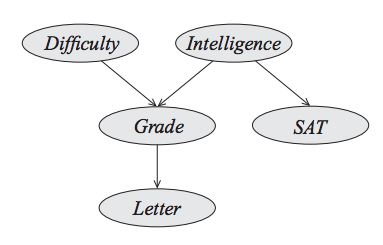
\includegraphics[scale=0.3]{pgm_eg}
		\end{figure}
	\begin{equation}
	\begin{aligned}
	p(l, g, i, d, s) = p(l \mid g) p(g \mid i, d) p(i) p(d) p(s\mid i)
	\end{aligned}
	\end{equation}
	
}



\frame[<+->]{
	\frametitle{Bayesian networks}
		\begin{itemize}
		\item Bayesian network is a directed graph  $G =(V , E)$ 
		\item  Together with a random variable $x_i$ for each node $i \in V$ 
		\item One conditional probability distribution (CPD) conditioned on its parents\\
		$p(x_i \mid x_{A_i})$
		\item probability  $p$ factorizes over a DAG  $G$  if it can be decomposed into a product of factors
		\end{itemize}
}

\frame[<+->]{
	\frametitle{Bayesian networks}
		\begin{figure}
		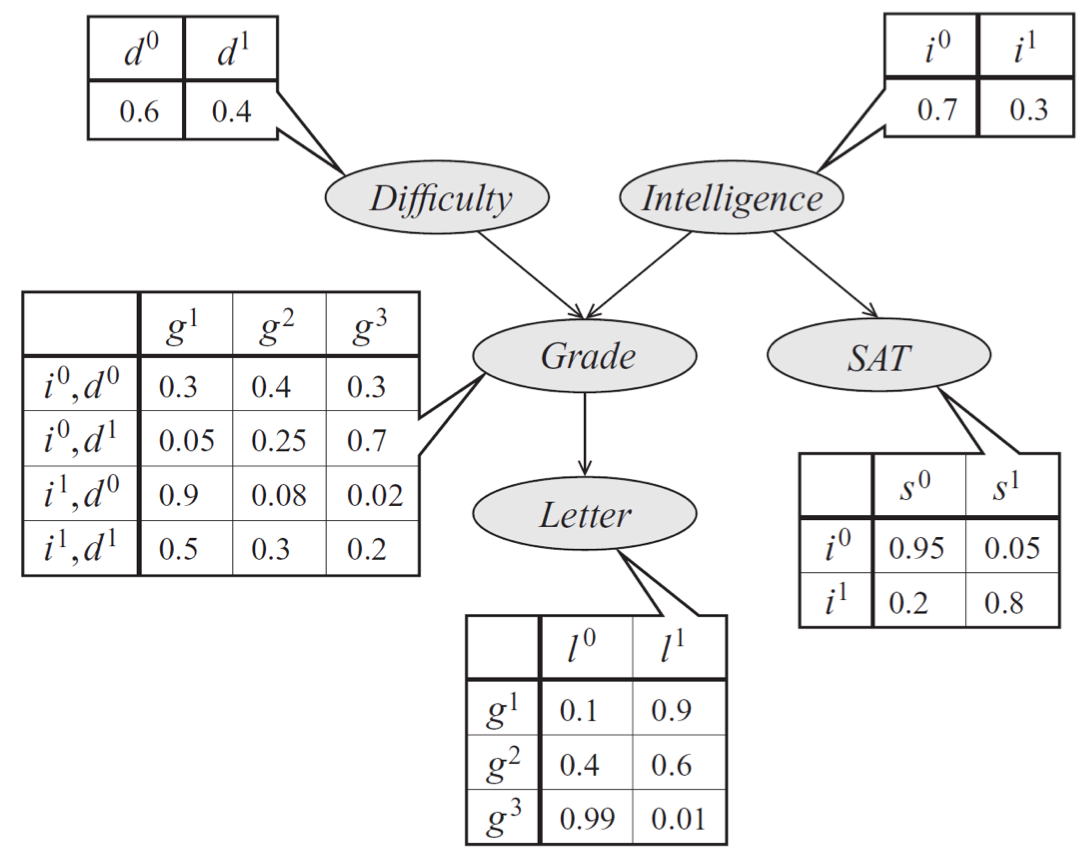
\includegraphics[scale=0.3]{grade-model}
		\end{figure}
	\begin{equation}
	\begin{aligned}
	p(l, g, i, d, s) = p(l \mid g) p(g \mid i, d) p(i) p(d) p(s\mid i)
	\end{aligned}
	\end{equation}
	
}

\frame[<+->]{
	\frametitle{Bayesian networks}
		\begin{figure}
		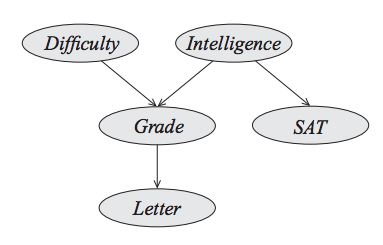
\includegraphics[scale=0.3]{pgm_eg}
		\end{figure}
%	\begin{equation}
	%\begin{aligned}
	
	%\end{aligned}
	%\end{equation}
	
}


\frame[<+->]{
	\frametitle{Probabilistic modelling}
	\begin{itemize}
	\item Inference \\
	Given a probabilistic model, how do we obtain answers to relevant questions about the world? \\
	Querying the marginal or conditional probabilities of certain events of interest.
		\begin{equation}
	\begin{aligned}
	p(x_1) = \sum_{x_2} \sum_{x_2}...\sum_{x_n} p(x_1, x_2, x3, ..., x_n)
	\end{aligned}
	\end{equation}
	\end{itemize}
	
}

\section{Introduction word alignment}

\frame[<+->]{
	\frametitle{Word alignment}
		\begin{itemize}
		\item  IBM models assume that each word in the French sentence is a translation of exactly zero or one word of the English sentence.
		 \item The notation to refer to each word.\\\
		  Let a French sentence $f$ be represented by an array of $m$ words, $\left \langle f_1, ..., f_m  \right \rangle$, \\
		  and English sentence $e$ be represented by an array of $l$ words, $\left \langle e_1, ..., e_l  \right \rangle$ 
		  \item IBM models decompose the joint probability of a sentence pair with the chain rule as:
		  \begin{equation}
			\begin{aligned}
				p(e_{1}^{l}, f_{1}^{m}) = \underbrace{p(e_{1}^{l})}_{\text{language model}} \times \underbrace{p(f_{1}^{m} \mid e_{1}^{l}) }_{\text{translation model}}
			\end{aligned}
		\end{equation}
		
		\item French words are conditionally independent given the English sentence.
		\item inference can be performed exactly.
		\item 
		  %\item The assumption that each French word aligned to exactly one English word \\
		  %We represent the alignment by an array $a$ of length $I$, denoted $\left \langle f_1, ..., f_I  \right \rangle$,
		  %\item  Alignment variable $a_i$ takes a value in the range $[0, J]$ denoting the index of the English word to which French word fi is aligned. \\
		%If $ai = 0$, this means that $f_i$ is not aligned to any word in the English sentence, called \cbleu{null alignment}. 
		\end{itemize}
}

\frame[<+->]{
	\frametitle{Mixture models}
		\begin{itemize}
		\item A mixture model consist of $c$ mixture components, each defines a distribution over the space $X$.
		\item Each component can specialise its distribution on a subset of the data.
		\item The probability of a mixture model with $c$ components assigns to $n$ data point is denoted by:
		
		\begin{equation}
			\begin{aligned}
				p(x_{1}^{n}) &=  \prod_{i=1}^{n} \sum_{j=1}^{c} p(x_i, y_i = j) \\
				&= \prod_{i=1}^{n} \sum_{j=1}^{c} p(y_i= j)p(x_i \mid y_i = j)
			\end{aligned}
		\end{equation}
		\item We introduced the random variable $y_i$ that ranges over the mixture components
		\begin{figure}
		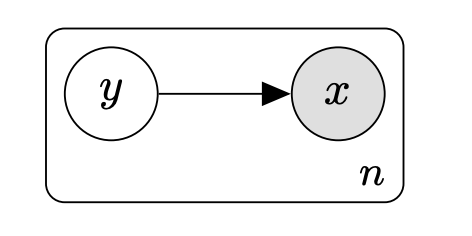
\includegraphics[scale=0.5]{mixture_pgm}
		\end{figure}
		\end{itemize}
}






\frame[<+->]{
	\frametitle{Word Alignment}
		\begin{itemize}
		\item  Learn a conditional probabilistic model of a French sentence $f$ given an English sentence $e$,\\
		 which we denote as  $p(f|e)$.
		 \item A dataset $D$ of $N$ sentence pairs that are known to be translations of each other, \\
		 $D = {(f^{(1)}, e^{(1)})...(f^{(N)}, e^{(N)})}$
		 \item  \cblue{Goal} of our model will be to uncover the hidden word-to-word correspondences in these
translation pairs.
		\item We will learn the model from data, and use it to predict the existence of the missing word alignments
		\end{itemize}
}





\frame[<+->]{
	\frametitle{Generative Process}
	\begin{itemize}
	\item 	Generative process for the French sentence conditioned on the English sentence:
		\begin{enumerate}
		\item Choose French sentence length $m$ based on the English sentence length $l$
		\item For each French position $j$, choose the English position $a_j$ that it is generated from
		\item For each French position $j$, choose a French word based on the English word in position $a_j$
		\end{enumerate}
	\item The generative story introduces the alignment variable $a_j$ \\
	It is an indicator for the mixture component that the French word in position $j$ is generated from
	\item The mixture components are English words
	\end{itemize}
}

\frame[<+->]{
	\frametitle{IBM graphical model}
		\begin{figure}
		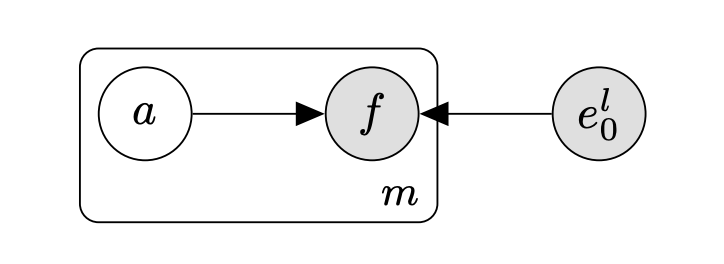
\includegraphics[scale=0.5]{ibm_pgm}
		\end{figure}
%	\begin{equation}
	%\begin{aligned}
	
	%\end{aligned}
	%\end{equation}
	
}





